\documentclass[a4paper,12pt]{report}

\usepackage{alltt, fancyvrb, url}
\usepackage{graphicx}
\usepackage[utf8]{inputenc}
\usepackage{float}
\usepackage{hyperref}

% Questo commentalo se vuoi scrivere in inglese.
\usepackage[italian]{babel}

\usepackage[italian]{cleveref}

\title{Relazione per\\``Programmazione ad Oggetti''}

\author{Nicolò Guerra \and
Emma Leonardi \and 
Filippo Casadei \and
Lorenzo Tagliani}
\date{\today}

\begin{document}

\maketitle

\tableofcontents

\chapter{Analisi}

Bubble Blaster è un gioco della categoria puzzle games, clone del gioco arcade Puzzle Bubble. Il gioco è formato da una schermata
rettangolare in cui vengono create file di bolle colorate che scendono dall'alto. Obiettivo del gioco è utilizzare il cannone 
posto in fondo alla schermata per formare gruppi di bolle dello stesso colore e farle così esplodere, cercando di ottenere il maggior
punteggio possibile. La partita è persa se le bolle arrivano in fondo allo schermo.  

\section{Requisiti}

\subsubsection{Requisiti funzionali}
\begin{itemize}
	\item All'apertura del gioco verrà mostrata una schermata per la scelta delle modalità di gioco e delle opzioni.
	\item Il gioco dovrà generare una griglia di bolle colorate in maniera casuale.
	\item Il cannone in basso dovrà permettere di sparare bolle generate casualmente, muovendosi angolarmente a destra e sinistra.
	\item Le bolle sparate dal cannone potranno rimbalzare sui muri del campo di gioco se colpiti.
	\item Le bolle dovranno scoppiare alla formazione di gruppi di almeno 3 bolle dello stesso colore adiacenti, facendo cadere eventuali altre bolle sottostanti senza ulteriori sostegni.
	\item Il gioco dovrà dare una schermata di game over se le palline raggiungono il fondo dello schermo.
	\item Il gioco dovrà gestire un punteggio.
\end{itemize}

\subsubsection{Requisiti non funzionali}
\begin{itemize}
    \item Il gioco dovrà fornire una esperienza fluida.
    \item Il gioco dovrà avere musica di sottofondo e effetti sonori per lo scoppio delle bolle e il game over.
\end{itemize}

\subsection{Requisiti facoltativi}
Questi requisiti non sono necessari al funzionamento di base del gioco e per questioni di tempistica potrebbero non essere implementati.
\begin{itemize}
    \item Salvataggio e caricamento della partita
    \item Gestione di una leaderboard con i punteggi migliori
    \item Effetti sonori e musica
    \item Preview della prossima pallina che verrà caricata sul cannone e possibilità di scambiarla con quella caricata
    \item Diversi livelli di difficoltà
    \item Animazioni fluide
    \item Modalità 2 giocatori
\end{itemize}

\section{Analisi e modello del dominio}

L'entità principale in gioco è la Bubble, un insieme di Bubble formano una Grid. Una Grid dovrà poter essere generata in maniera casuale.
Una bolla potrà essere sparata da un cannone, il quale potrà anche decidere di scambiarla con la successiva. Lo scoppio delle bolle dovrà inoltre far incrementare il punteggio.

\begin{figure}[H]
\centering{}
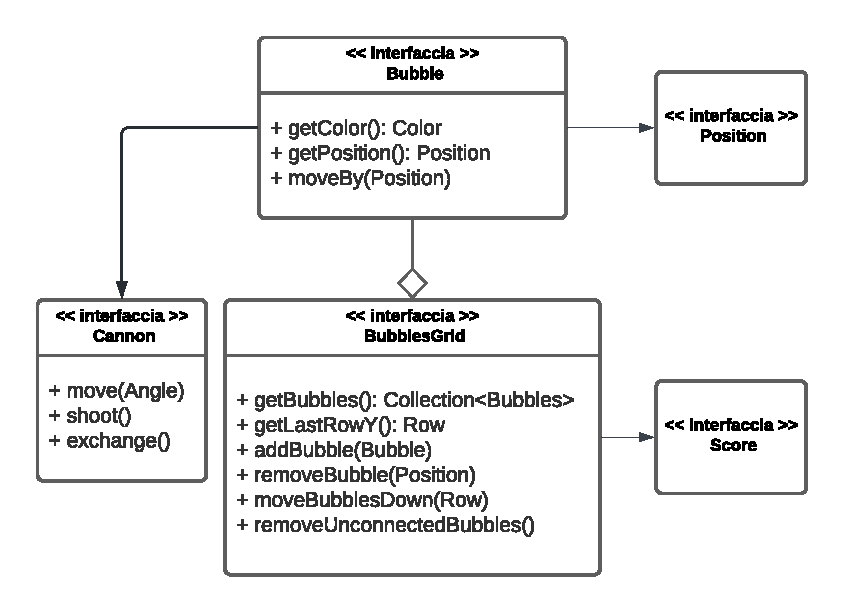
\includegraphics{img/analysis.pdf}
\caption{UML delle entità che rappresentano il dominio del problema.}
\label{img:analysis}
\end{figure}

\chapter{Design}

\section{Architettura}

Per questo progetto è stato scelto di fare uso del pattern MVC, che consente di separare in maniera efficace la logica del dominio da quella di visualizzazione e interazione con l'utente. 
L'interfaccia principale del Model è rappresentata dal Level che fornisce le informazioni necessarie alla rappresentazione di una partita. La view è nascosta da un interfaccia che non dipende dalla sua 
implementazione, in questo modo una sua sostituzione in blocco non dovrebbe comportare modifiche al resto dell'architettura dell'applicazione, questo perché il modello non è in alcun modo a conoscenza 
di come venga rappresentato all'esterno. 
%
Il punto d'ingresso del Model è il Cannon, che permette al Controller di modificare lo stato del gioco muovendo il cannone e sparando le bolle.
Il tempo del gioco è scandito dal Controller. Il movimento del cannone è invece un evento generato dalla View, che viene passato al Model attraverso il controller e gestito in maniera asincrona.

\begin{figure}[h]
\centering{}
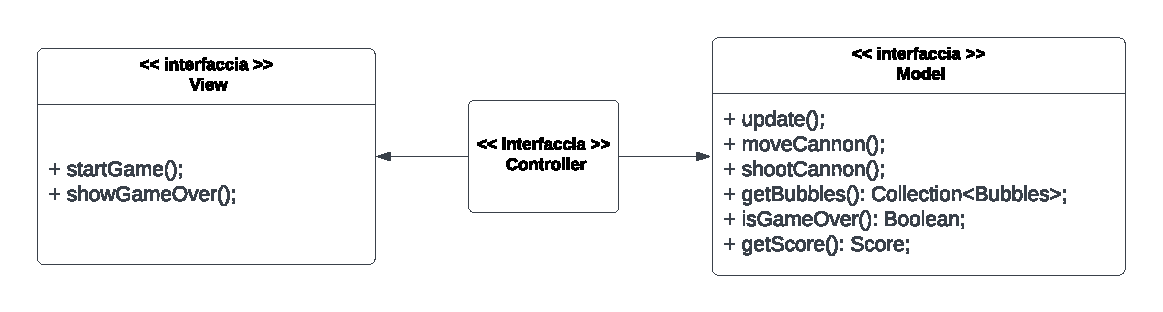
\includegraphics[width=\textwidth]{img/arch.pdf}
\caption{Schema UML architetturale del gioco. L'interfaccia \texttt{Controller} gestisce il flusso dell'applicazione, mentre la \texttt{View} gestisce l'interazione con l'utente e il \texttt{Model} fornisce le informazioni sul \texttt{Level}.}
\end{figure}

\section{Design dettagliato}
\subsection{Nicolò Guerra}
\subsubsection{Caratteristiche della griglia di bolle}

\begin{figure}[H]
\centering{}
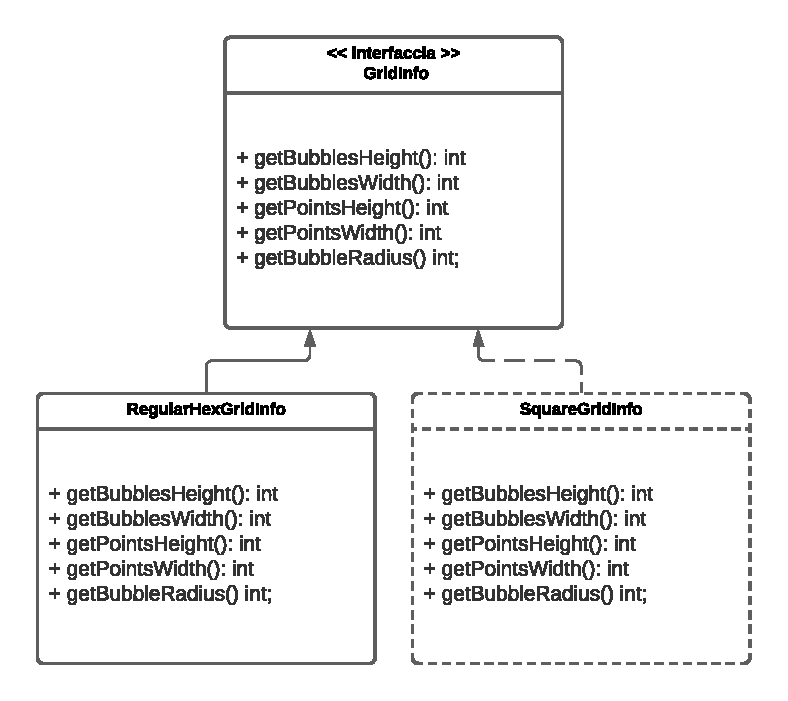
\includegraphics[width=\textwidth]{img/strategy_gridinfo.pdf}
\caption{Rappresentazione UML dell'oggetto GridInfo}
\end{figure}

\paragraph{Problema} Potenzialmente il gioco può gestire più tipi di griglie diverse per quanto riguarda dimensioni, forme delle caselle e altre caratteristiche, il che può portare a disallineamenti e incoerenze
tra parti diverse del modello, oltre a una difficoltà di rappresentazione delle bolle nello spazio da parte della View, che non conosce griglie o altre entità specifiche del Model.

\paragraph{Soluzione} Le caratteristiche della griglia vengono fornite da una interfaccia di tipo GridInfo implementata come \textit{Strategy}, in questo caso ad esempio la RegularHexGridInfo viene 
inizializzata con le dimensioni in bolle della griglia e si occupa autonomamente di effettuare i calcoli necessari per avere una griglia di esagoni regolari. Un'ulteriore implementazione potrebbe essere 
ad'esempio una SquareGridInfo che fornisce informazioni per una griglia a celle quadrate.

\subsubsection{Gestione del GameOver}

\begin{figure}[H]
\centering{}
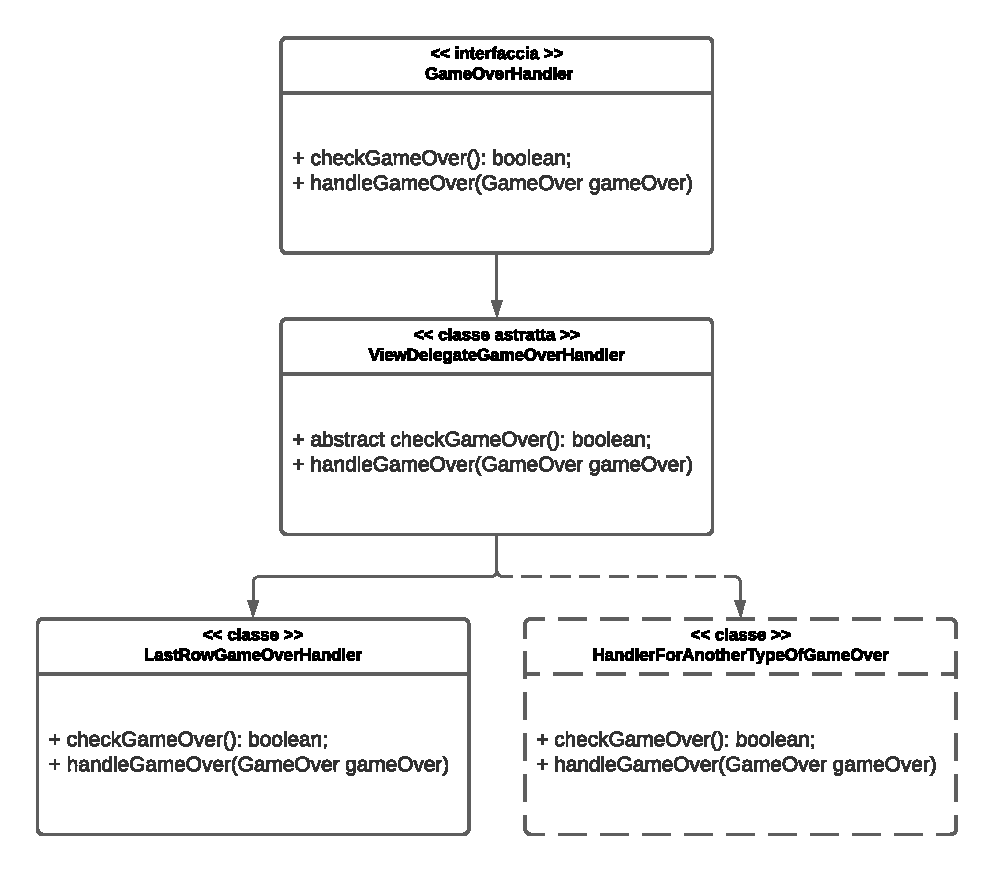
\includegraphics[width=\textwidth]{img/gameover.pdf}
\caption{Rappresentazione UML del gestore dei GameOver}
\end{figure}

\paragraph{Problema} I GameOver potrebbero essere generati in modi diversi (tempo scaduto, raggiungimento dell'ultima riga...) e voler essere gestiti in maniera diversa.

\paragraph{Soluzione} Un interfaccia GameOverHandler con 2 metodi per controllare se è avvenuto un GameOver e per gestirlo, implementando questa interfaccia è possibile definire quando avviene un GameOver 
e come questo venga gestito. Per separare ulteriormente controllo e gestione una classe astratta ViewDelegateGameOverHandler che implementa la gestione passando l'evento di gameover alla View, e con un metodo
astratto per controllare se è accaduto un gameover. Quest'ultimo viene implementato dalla sottoclasse LastRowGameOverHandler, la quale non fa altro che controllare se le bolle nella griglia hanno raggiunto l'ultima 
riga.

\subsubsection{Salvataggio su file}

\begin{figure}[H]
\centering{}
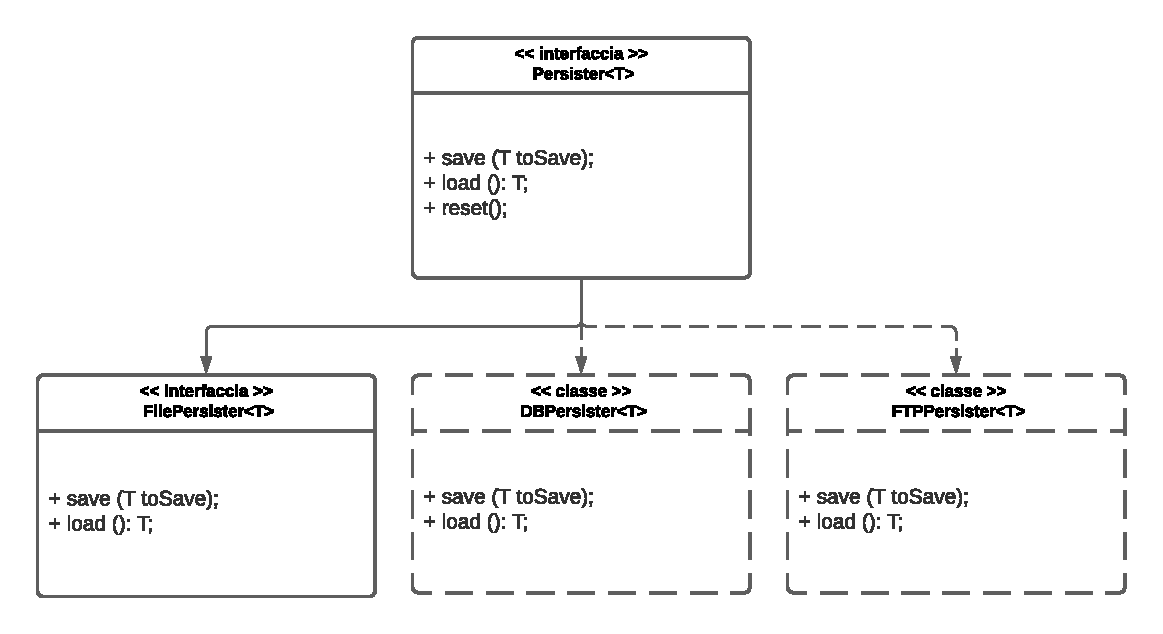
\includegraphics[width=.7\textwidth]{img/persister.pdf}
\caption{Strategy per un oggetto che salva oggetti}
\end{figure}

\paragraph{Problema} Spesso l'applicazione ha necessita di salvare lo stato di alcuni suoi oggetti per poi recuperarlo in un secondo momento.

\paragraph{Soluzione} Per poter salvare lo stato di oggetti diversi su disco ho creato un interfaccia generica persister che fa da strategy, con un metodo per salvare un oggetto e un metodo per leggerlo. 
L'implementazione di questa nasconde all'utilizzatore il modo in cui vengono persistiti. Si possono quindi creare ad esempio diverse implementazioni che salvano su file, su database o in cloud implementando i 
metodi read e write. Rispettando la stessa interfaccia le sottoclassi diventano intercambiabili tra di loro.

\subsubsection{Caricamento degli assets della View}

\begin{figure}[H]
\centering{}
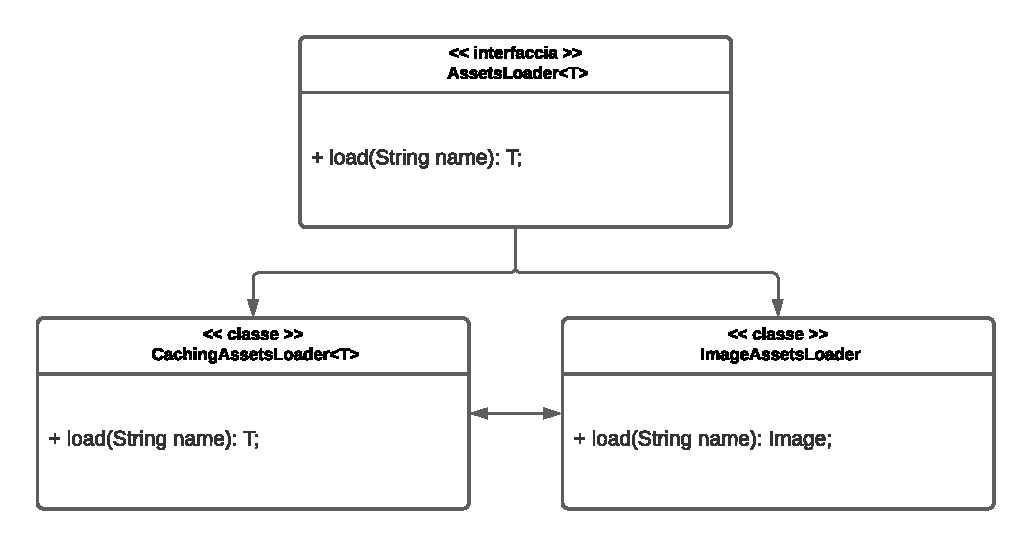
\includegraphics[width=.7\textwidth]{img/assetsloader}
\caption{Decorator per cache di un assets loader}
\end{figure}

\paragraph{Problema} L'implementazione grafica della View ha bisogno che le vengano forniti gli assets del gioco come le figure delle bolle e del cannone. Deve essere un caricamento efficiente perché gli assets
possono anche essere richiesti più volte al secondo.

\paragraph{Soluzione} Per delegare il caricamento degli assets a un altro componente è stata creata l'interfaccia AssetsLoader che ha un metodo in grado di caricare un assets la cui implementazione
non è specificata. Una classe StandardAssetsLoader carica gli assets dalla cartella resources su richiesta e un CachedAssetsLoader la wrappa implementando un meccanismo di cache per ridurre gli accessi a disco
e aumentarne l'efficienza. In questo modo è facile riutilizzare il meccanismo di cache per un AssetsLoader che carica altri tipi di assets.

\subsubsection{Gestione del tempo di gioco}

\begin{figure}[H]
\centering{}
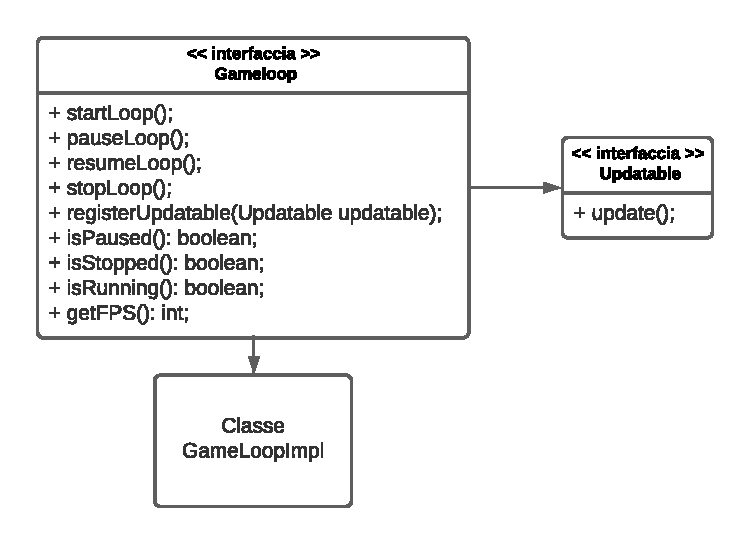
\includegraphics[width=.7\textwidth]{img/gameloop.pdf}
\caption{UML del Gameloop}
\end{figure}

\paragraph{Problema} Il gioco ha bisogno di essere aggiornato a intervalli regolari, ad esempio per gestire il movimento delle palline o per far ridisegnare la View.

\paragraph{Soluzione} È stato utilizzato il pattern Gameloop, creando un interfaccia che ne definisce le interazioni con il Controller, presso cui altri componenti che implementano Updatable possono registrarsi 
per essere aggiornati ad ogni ciclo.

\chapter{Sviluppo}
\section{Testing automatizzato}

Il testing automatizzato è un requisito di qualunque progetto software che si rispetti, e consente di verificare che non vi siano regressioni nelle funzionalità a fronte di aggiornamenti.
%
Per quanto riguarda questo progetto è considerato sufficiente un test minimale, a patto che sia completamente automatico.
%
Test che richiedono l'intervento da parte dell'utente sono considerati \textit{negativamente} nel computo del punteggio finale.

\subsection*{Elementi positivi}

\begin{itemize}
 \item Si descrivono molto brevemente i componenti che si è deciso di sottoporre a test automatizzato.
 \item Si utilizzano suite specifiche (e.g. JUnit) per il testing automatico.
 \item Se sono stati eseguiti test manuali di rilievo, si elencano descrivendo brevemente la ragione per cui non sono stati automatizzati. Ad esempio, se tutto il team sviluppa e testa su uno stesso sistema operativo e si sono svolti test manuali per verificare, ad esempio, il corretto funzionamento dell'interfaccia grafica o di librerie native su altri sistemi operativi, può avere senso menzionare la cosa.
\end{itemize}

\section{Metodologia di lavoro}

Ci aspettiamo, leggendo questa sezione, di trovare conferma alla divisione operata nella sezione del design di dettaglio, e di capire come è stato svolto il lavoro di integrazione.
%
\textbf{Andrà realizzata una sotto-sezione separata per ciascuno studente} che identifichi le porzioni di progetto sviluppate, separando quelle svolte in autonomia da quelle sviluppate in collaborazione.
%
Diversamente dalla sezione di design, in questa è consentito elencare package/classi, se lo studente ritiene sia il modo più efficace di convogliare l'informazione.
%
Si ricorda che l'impegno deve giustificare circa 40-50 ore di sviluppo (è normale e fisiologico che approssimativamente la metà del tempo sia impiegata in analisi e progettazione).

\subsection*{Elementi positivi}

\begin{itemize}
	\item Si identifica con precisione il ruolo di ciascuno all'interno del gruppo, ossia su quale parte del progetto ciascuno dei componenti si è concentrato maggiormente.
	\item La divisione dei compiti è equa, ossia non vi sono membri del gruppo che hanno svolto molto più lavoro di altri.
	\item La divisione dei compiti è coerente con quanto descritto nelle parti precedenti della relazione.
	\item La divisione dei compiti è realistica, ossia le dipendenze fra le parti sviluppate sono minime.
	\item Si identifica quale parte del software è stato sviluppato da tutti i componenti insieme.
	\item Si spiega in che modo si sono integrate le parti di codice sviluppate separatamente, evidenziando eventuali problemi. Ad esempio, una strategia è convenire sulle interfacce da usare (ossia, occuparsi insieme di stabilire l'architettura) e quindi procedere indipendentemente allo sviluppo di parti differenti. Una possibile problematica potrebbe essere una dimenticanza in fase di design architetturale che ha costretto ad un cambio e a modifiche in fase di integrazione. Una situazione simile è la norma nell'ingegneria di un sistema software non banale, ed il processo di progettazione top-down con raffinamento successivo è il così detto processo ``a spirale''.
	\item Si descrive in che modo è stato impiegato il DVCS.
\end{itemize}

\subsection*{Elementi negativi}
\begin{itemize}
	\item Non si chiarisce chi ha fatto cosa.
	\item C'è discrepanza fra questa sezione e le sezioni che descrivono il design dettagliato.
	\item Tutto il progetto è stato svolto lavorando insieme invece che assegnando una parte a ciascuno.
	\item Non viene descritta la metodologia di integrazione delle parti sviluppate indipendentemente.
	\item Uso superficiale del DVCS.
\end{itemize}

\section{Note di sviluppo}

Questa sezione, come quella riguardante il design dettagliato va svolta \textbf{singolarmente da ogni membro del gruppo}.

Ciascuno dovrà mettere in evidenza eventuali particolarità del suo metodo di sviluppo, ed in particolare:
\begin{itemize}
	\item \textbf{Elencare} (fare un semplice elenco per punti, non un testo!) le feature \textit{avanzate} del linguaggio e dell'ecosistema Java che sono state
utilizzate. Le feature di interesse sono:
	\begin{itemize}
		\item Progettazione con generici, ad esempio costruzione di nuovi tipi generici, e uso di generici bounded. Uso di classi generiche di libreria non è considerato avanzato.
		\item Uso di lambda expressions
		\item Uso di \texttt{Stream}, di \texttt{Optional} o di altri costrutti funzionali
		\item Uso della reflection
		\item Definizione ed uso di nuove annotazioni
		\item Uso del Java Platform Module System
		\item Uso di parti di libreria non spiegate a lezione (networking, compressione, parsing XML, eccetera...)
		\item Uso di librerie di terze parti (incluso JavaFX): Google Guava, Apache Commons...
		\item Uso di build systems
	\end{itemize}
	Si faccia molta attenzione a non scrivere banalità, elencando qui features di tipo ``core'', come le eccezioni, le enumerazioni, o le inner class: nessuna di queste è considerata avanzata.
	\item Descrivere \textit{molto brevemente} le librerie utilizzate nella propria parte di progetto, se non trattate a lezione (ossia, se librerie di terze parti e/o se componenti del JDK non visti, come le socket). Si ricorda che l'utilizzo di librerie è valutato \emph{positivamente}.
	\item Sviluppo di algoritmi particolarmente interessanti \emph{non forniti da alcuna libreria} (spesso può convenirvi chiedere sul forum se ci sia una libreria per fare una certa cosa, prima di gettarvi a capofitto per scriverla voi stessi).
\end{itemize}
%
In questa sezione, \textit{dopo l'elenco}, è anche bene evidenziare eventuali pezzi di codice ``riadattati'' (o scopiazzati...) da Internet o da altri progetti, pratica che tolleriamo ma che non raccomandiamo.
%
I pattern di design, invece \textbf{non} vanno messi qui.
%
L'uso di pattern di design (come suggerisce il nome) è un aspetto avanzato di design, non di implementazione,
e non va in questa sezione.

\subsection*{Elementi positivi}

\begin{itemize}
	\item Si elencano gli aspetti avanzati di linguaggio che sono stati impiegati
	\item Si elencano le librerie che sono state utilizzate
	\item Si descrivono aspetti particolarmente complicati o rilevanti relativi all'implementazione,
ad esempio, in un'applicazione performance critical, un uso particolarmente avanzato di meccanismi
di caching, oppure l'implementazione di uno specifico algoritmo.
	\item Se si è utilizzato un particolare algoritmo, se ne cita la fonte originale. Ad esempio, se
si è usato Mersenne Twister per la generazione dei numeri pseudo-random, si cita \cite{mersenne}.
	\item Si identificano parti di codice prese da altri progetti, dal web, o comunque scritte in forma originale da altre persone. In tal senso, si ricorda che agli ingegneri non è richiesto di re-inventare la ruota continuamente: se si cita debitamente la sorgente è tollerato fare uso di di snippet di codice per risolvere velocemente problemi non banali. Nel caso in cui si usino snippet di codice di qualità discutibile, oltre a menzionarne l'autore originale si invitano gli studenti ad adeguare tali parti di codice agli standard e allo stile del progetto. Contestualmente, si fa presente che è largamente meglio fare uso di una libreria che copiarsi pezzi di codice: qualora vi sia scelta (e tipicamente c'è), si preferisca la prima via.
\end{itemize}

\subsection*{Elementi negativi}
\begin{itemize}
	\item Si elencano feature core del linguaggio invece di quelle segnalate. Esempi di feature
core da non menzionare sono:
    \begin{itemize}
        \item eccezioni;
        \item classi innestate;
        \item enumerazioni;
        \item interfacce.
    \end{itemize}
	\item Si elencano applicazioni di terze parti (peggio se per usarle occorre licenza, e lo
studente ne è sprovvisto) che non c'entrano nulla con lo sviluppo, ad esempio:
    \begin{itemize}
        \item Editor di grafica vettoriale come Inkscape o Adobe Illustrator;
        \item Editor di grafica scalare come GIMP o Adobe Photoshop;
        \item Editor di audio come Audacity;
        \item Strumenti di design dell'interfaccia grafica come SceneBuilder: il codice è in ogni caso inteso come sviluppato da voi.
    \end{itemize}
	\item Si descrivono aspetti di scarsa rilevanza, o si scende in dettagli inutili.
	\item Sono presenti parti di codice sviluppate originalmente da altri che non vengono
debitamente segnalate. In tal senso, si ricorda agli studenti che i docenti hanno accesso a tutti i
progetti degli anni passati, a Stack Overflow, ai principali blog di sviluppatori ed esperti Java (o sedicenti tali), ai blog dedicati allo sviluppo di soluzioni e applicazioni (inclusi blog dedicati ad Android e allo sviluppo di videogame), nonché ai social network. Conseguentemente, è \emph{molto} conveniente \emph{citare} una fonte ed usarla invece di tentare di spacciare per proprio il lavoro di altri.
	\item Si elencano design pattern
\end{itemize}

\chapter{Commenti finali}

In quest'ultimo capitolo si tirano le somme del lavoro svolto e si delineano eventuali sviluppi
futuri.

\textit{Nessuna delle informazioni incluse in questo capitolo verrà utilizzata per formulare la valutazione finale}, a meno che non sia assente o manchino delle sezioni obbligatorie.
%
Al fine di evitare pregiudizi involontari, l'intero capitolo verrà letto dai docenti solo dopo aver formulato la valutazione.

\section{Autovalutazione e lavori futuri}

\textbf{È richiesta una sezione per ciascun membro del gruppo, obbligatoriamente}.
%
Ciascuno dovrà autovalutare il proprio lavoro, elencando i punti di forza e di debolezza in quanto prodotto.
Si dovrà anche cercare di descrivere \emph{in modo quanto più obiettivo possibile} il proprio ruolo all'interno del gruppo.
Si ricorda, a tal proposito, che ciascuno studente è responsabile solo della propria sezione: non è un problema se ci sono opinioni contrastanti, a patto che rispecchino effettivamente l'opinione di chi le scrive.
Nel caso in cui si pensasse di portare avanti il progetto, ad esempio perché effettivamente impiegato, o perché sufficientemente ben riuscito da poter esser usato come dimostrazione di esser capaci progettisti, si descriva brevemente verso che direzione portarlo.

\section{Difficoltà incontrate e commenti per i docenti}

Questa sezione, \textbf{opzionale}, può essere utilizzata per segnalare ai docenti eventuali problemi o difficoltà incontrate nel corso o nello svolgimento del progetto, può essere vista come una seconda possibilità di valutare il corso (dopo quella offerta dalle rilevazioni della didattica) avendo anche conoscenza delle modalità e delle difficoltà collegate all'esame, cosa impossibile da fare usando le valutazioni in aula per ovvie ragioni.
%
È possibile che alcuni dei commenti forniti vengano utilizzati per migliorare il corso in futuro: sebbene non andrà a vostro beneficio, potreste fare un favore ai vostri futuri colleghi.
%
Ovviamente \textit{il contenuto della sezione non impatterà il voto finale}.

\appendix
\chapter{Guida utente}

Capitolo in cui si spiega come utilizzare il software. Nel caso in cui il suo uso sia del tutto
banale, tale capitolo può essere omesso.
%
A tal riguardo, si fa presente agli studenti che i docenti non hanno mai utilizzato il software
prima, per cui aspetti che sembrano del tutto banali a chi ha sviluppato l'applicazione possono non
esserlo per chi la usa per la prima volta.
%
Se, ad esempio, per cominciare una partita con un videogioco è necessario premere la barra
spaziatrice, o il tasto ``P'', è necessario che gli studenti lo segnalino.

\subsection*{Elementi positivi}

\begin{itemize}
 \item Si istruisce in modo semplice l'utente sull'uso dell'applicazione, eventualmente facendo uso di schermate e descrizioni.
\end{itemize}

\subsection*{Elementi negativi}
\begin{itemize}
 \item Si descrivono in modo eccessivamente minuzioso tutte le caratteristiche, anche minori, del software in oggetto.
 \item Manca una descrizione che consenta ad un utente qualunque di utilizzare almeno le funzionalità primarie dell'applicativo.
\end{itemize}

\chapter{Esercitazioni di laboratorio}

In questo capitolo ciascuno studente elenca gli esercizi di laboratorio che ha svolto
(se ne ha svolti),
elencando i permalink dei post sul forum dove è avvenuta la consegna.

\section*{Esempio}

\subsection{Paolino Paperino}

\begin{itemize}
 \item Laboratorio 04: \url{https://virtuale.unibo.it/mod/forum/discuss.php?d=12345#p123456}
 \item Laboratorio 06: \url{https://virtuale.unibo.it/mod/forum/discuss.php?d=22222#p222222}
 \item Laboratorio 09: \url{https://virtuale.unibo.it/mod/forum/discuss.php?d=99999#p999999}
\end{itemize}

\subsection{Paperon De Paperoni}

\begin{itemize}
 \item Laboratorio 04: \url{https://virtuale.unibo.it/mod/forum/discuss.php?d=12345#p123456}
 \item Laboratorio 05: \url{https://virtuale.unibo.it/mod/forum/discuss.php?d=22222#p222222}
 \item Laboratorio 06: \url{https://virtuale.unibo.it/mod/forum/discuss.php?d=99999#p999999}
 \item Laboratorio 07: \url{https://virtuale.unibo.it/mod/forum/discuss.php?d=22222#p222222}
 \item Laboratorio 08: \url{https://virtuale.unibo.it/mod/forum/discuss.php?d=99999#p999999}
 \item Laboratorio 09: \url{https://virtuale.unibo.it/mod/forum/discuss.php?d=22222#p222222}
 \item Laboratorio 10: \url{https://virtuale.unibo.it/mod/forum/discuss.php?d=99999#p999999}
 \item Laboratorio 11: \url{https://virtuale.unibo.it/mod/forum/discuss.php?d=22222#p222222}
\end{itemize}


\bibliographystyle{alpha}
\bibliography{13-template}

\end{document}